\documentclass[letter, 11pt]{article}
%% ================================
%% Packages =======================
\usepackage[utf8]{inputenc}      %%
\usepackage[T1]{fontenc}         %%
\usepackage{lmodern}             %%
\usepackage[spanish]{babel}      %%
\usepackage{fullpage}            %%
\usepackage{fancyhdr}            %%
\usepackage{graphicx}            %%
\usepackage{amsmath}             %%
\usepackage{color}               %%
\usepackage{mdframed}            %%
\usepackage[colorlinks]{hyperref}%%
\usepackage{wrapfig}             %%
%% ================================
%% ================================

%% ================================
%% Page size/borders config =======
\setlength{\oddsidemargin}{0in}  %%
\setlength{\evensidemargin}{0in} %%
\setlength{\marginparwidth}{0in} %%
\setlength{\marginparsep}{0in}   %%
\setlength{\voffset}{-0.5in}     %%
\setlength{\hoffset}{0in}        %%
\setlength{\topmargin}{0in}      %%
\setlength{\headheight}{54pt}    %%
\setlength{\headsep}{1em}        %%
\setlength{\textheight}{8.5in}   %%
\setlength{\footskip}{0.5in}     %%
%% ================================
%% ================================

%% =============================================================
%% Headers setup, environments, colors, etc.
%%
%% Header ------------------------------------------------------
\fancypagestyle{firstpage}
{
  \fancyhf{}
  \lhead{
\includegraphics[height=4.5em]{LogoDFI.jpg}}
  \rhead{FI3104-1 \semestre\\
         Métodos Numéricos para la Ciencia e Ingeniería\\
         Prof.: \profesor}
  \fancyfoot[C]{\thepage}
}

\pagestyle{plain}
\fancyhf{}
\fancyfoot[C]{\thepage}
%% -------------------------------------------------------------
%% Environments -------------------------------------------------
\newmdenv[
  linecolor=gray,
  fontcolor=gray,
  linewidth=0.2em,
  topline=false,
  bottomline=false,
  rightline=false,
  skipabove=\topsep
  skipbelow=\topsep,
]{ayuda}
%% -------------------------------------------------------------
%% Colors ------------------------------------------------------
\definecolor{gray}{rgb}{0.5, 0.5, 0.5}
%% -------------------------------------------------------------
%% Aliases ------------------------------------------------------
\newcommand{\scipy}{\texttt{scipy}}
%% -------------------------------------------------------------
%% =============================================================
%% =============================================================================
%% CONFIGURACION DEL DOCUMENTO =================================================
%% Llenar con la información pertinente al curso y la tarea
%%
\newcommand{\tareanro}{04}
\newcommand{\fechaentrega}{18/10/2016 23:59 hrs}
\newcommand{\semestre}{2018B}
\newcommand{\profesor}{Valentino González}
%% =============================================================================
%% =============================================================================


\begin{document}
\thispagestyle{firstpage}

\begin{center}
  {\uppercase{\LARGE \bf Tarea \tareanro}}\\
  Fecha de entrega: \fechaentrega
\end{center}


%% =============================================================================
%% ENUNCIADO ===================================================================

\begin{wrapfigure}{r}{0.3\textwidth}
  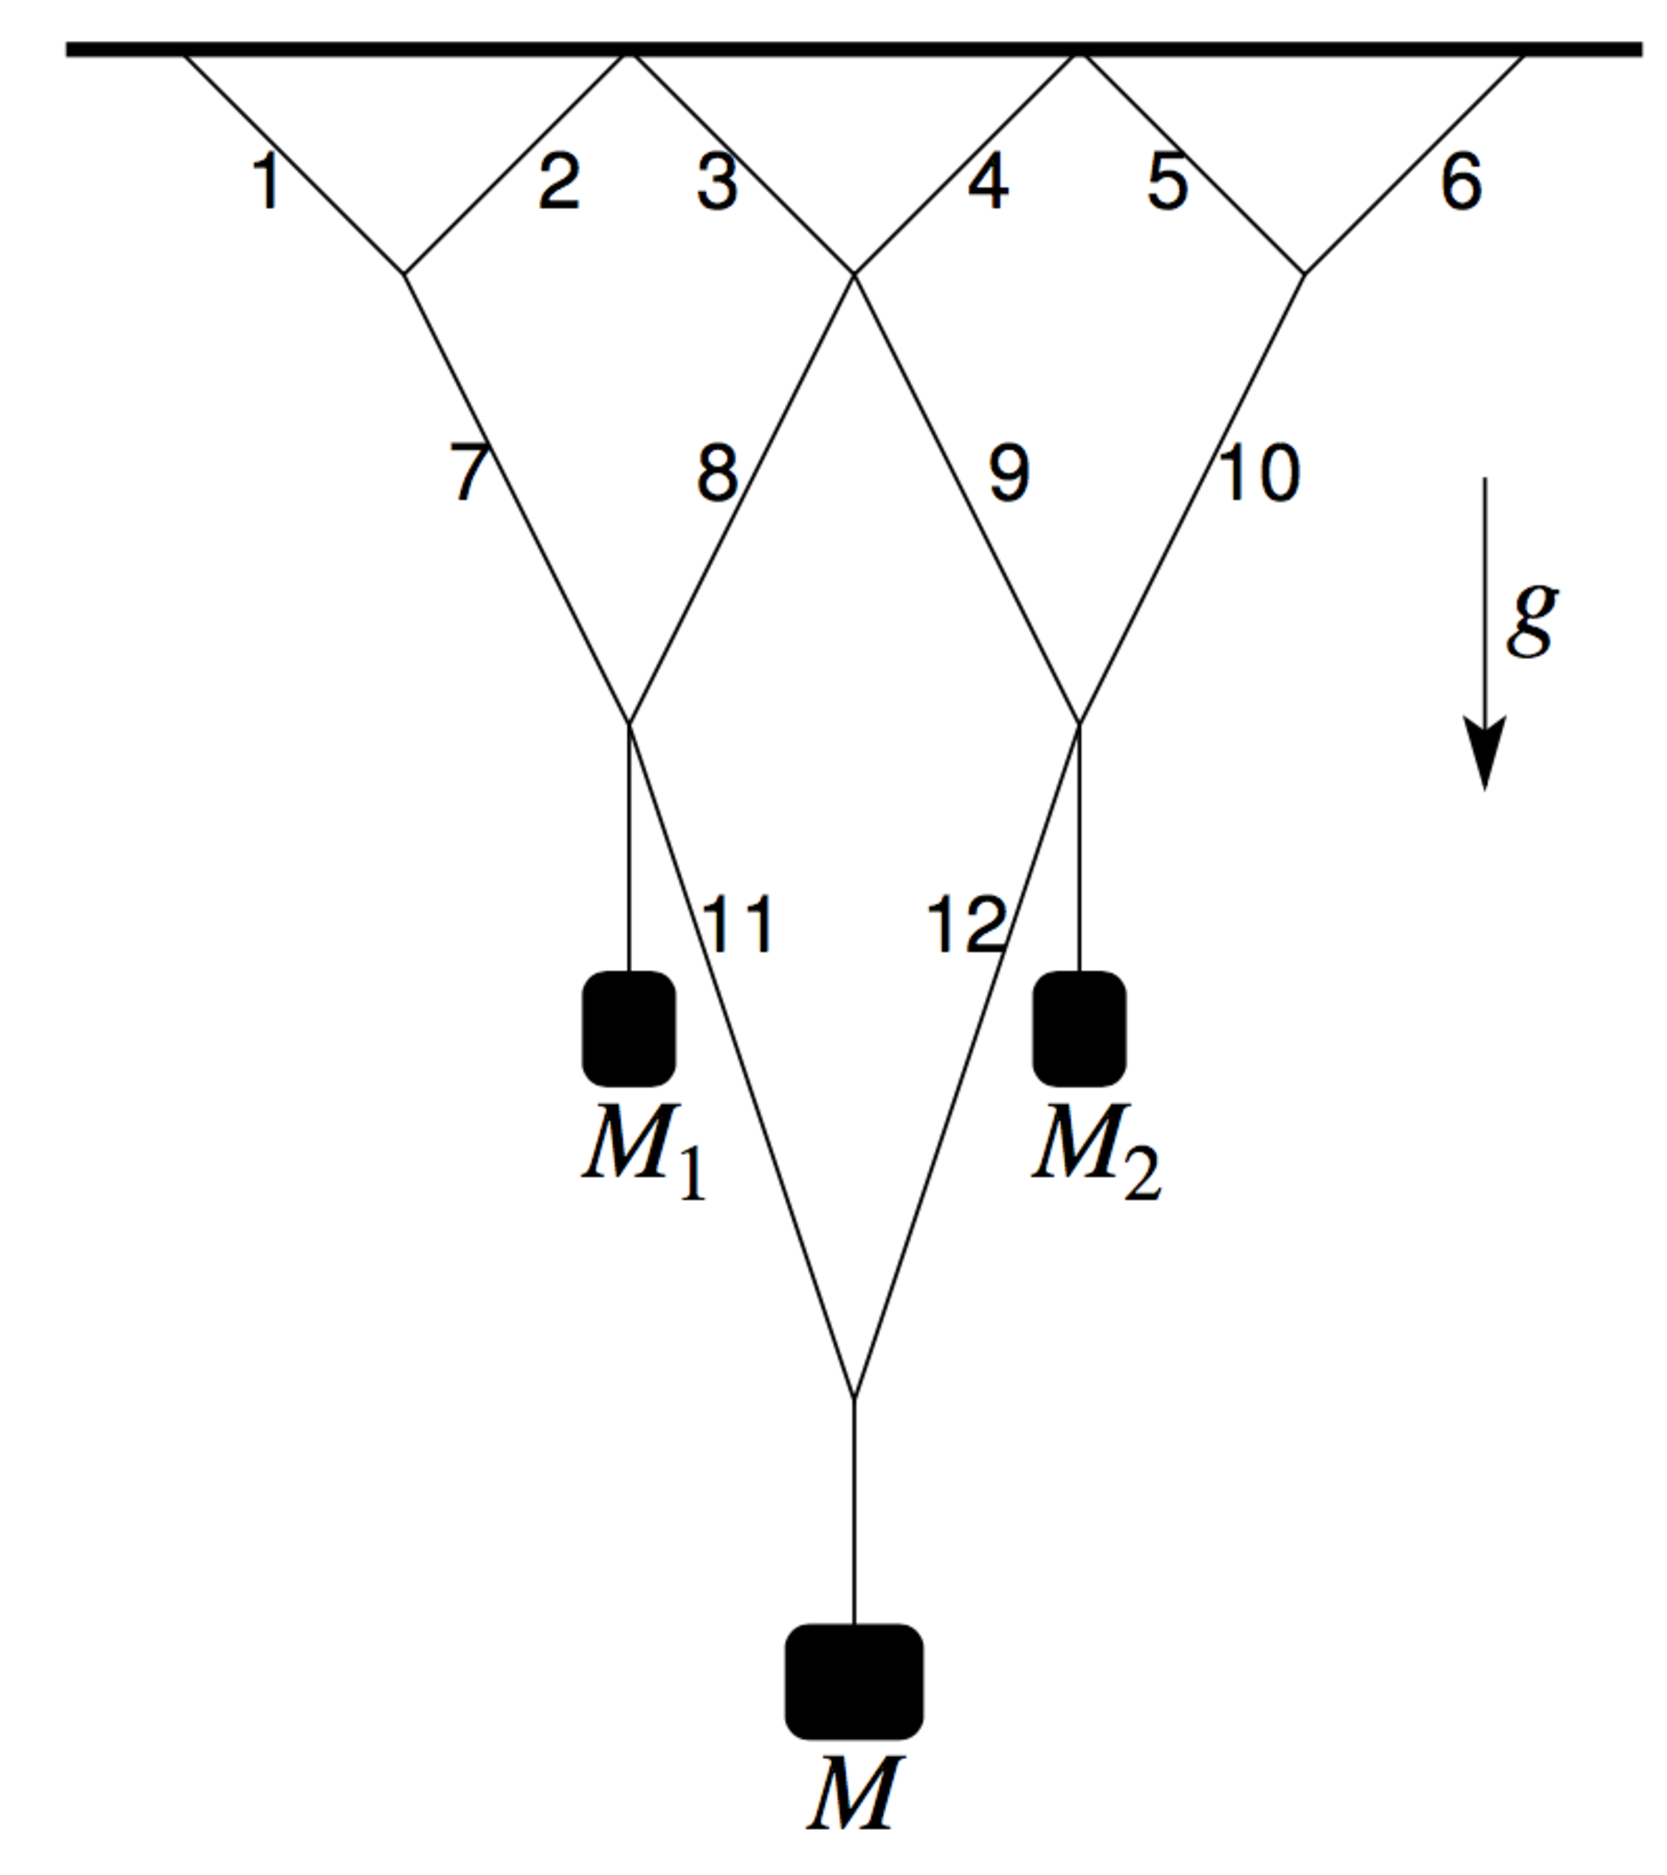
\includegraphics[width=0.28\textwidth]{12cuerdas.pdf}
\end{wrapfigure}

\noindent{\large \bf Problema}

\vskip 1.0em
Considere el sistema de cuerdas mostrado en la figura. Las cuerdas rotuladas de
1 a 12 son cuerdas ideales sujetas al techo y entre ellas para sostener tres
pesos de masas $M, M_1$ y $M_2$. Los largos de las cuerdas son tales que con
respecto a la vertical todas ellas forman ángulos $\pi/4$ en el primer nivel,
$\pi/6$ en el segundo nivel y $\pi/12$ en el último nivel (contando de arriba a
abajo).

\vskip 0.5em
Se busca determinar las tensiones en las 12 cuerdas, averiguar cuál es la
cuerda más tensa y cómo se comporta la tensión máxima en función de $M_1$. Para
esto, es necesario plantear las ecuaciones de balance de fuerzas en cada una de
las uniones de las cuerdas. A través de este procedimiento se obtienen 12
ecuaciones lineales (6 en la componente vertical y 6 en la horizontal).

\vskip 0.5em
\begin{itemize}
  \item Plantee el sistema de ecuaciones y representelo en la forma matricial:
    \begin{equation}
      A\ \vec{T} = \vec{b}
      \label{eq:eqlineal}
    \end{equation}
    donde $\vec{T}$ es el vector de las tensiones, $(T_1, ..., T_{12})^t$.

  \item La masa $M_2=1\,$kg y la masa $M=4.RRR\,$kg (donde $RRR$ son los
    últimos 3 dígitos de su RUT antes del dígito verificador). En tanto, la
    masa $M_1$ es un parámetro libre entre 0 y 2 kg. El objetivo del problema
    es determinar la tensión máxima del sistema como función del parámetro
    $M_1$.

  \item Para resolver el problema es necesario encontrar la solución a la
    ecuación \ref{eq:eqlineal} con la matriz $A$ que Ud.  determinó al
    comienzo.  La tarea pide resolver este problema de tres formas distintas
    para comparar su eficiencia:

    \begin{enumerate}
      \item Primero resuelva la ecuación \ref{eq:eqlineal} para cada valor de
        $M_1$ que Ud. explore. Utilice un método general (por ejemplo,
        eliminación de Gauss).

      \item Ahora utilizaremos el hecho de que la matriz $A$ no depende de
        $M_1$.  Cuando $M_1$ cambia, sólo cambia el lado derecho de la ecuación
        \ref{eq:eqlineal}. En éstos casos, puede ser más eficiente hacer una
        descomposición LU (o PLU) de $A$ una sola vez al principio y luego usar
        métodos específicos para resolver las ecuaciones con matrices
        \emph{triangulares} para cada valor de $M_1$.

      \item Por último, dado que $A$ no depende de $M_1$, intente calcular la
        inversa de la matriz una sola vez y luego resuelva la ecuación
        \ref{eq:eqlineal} para cada valor de $M_1$ multiplicando ambos lados
        por $A^{-1}$ cada vez.
    \end{enumerate}

  \item Compare la eficiencia de los 3 métodos descritos en términos de
    velocidad de ejecución. ¿A qué cree que se deben las diferencias
    observadas?

\end{itemize}

\begin{ayuda}
  \small
  \noindent {\bf Nota.}

  En su informe enfatice 2 aspectos: i) la resolución del problema, es decir,
  cómo se comporta $T_{\rm max}$ como función de $M_1$; y ii) la comparación de
  eficiencia de los 3 métodos utilizados.

\end{ayuda}

\begin{ayuda}
  \small
  \noindent {\bf Ayuda.}

  Hay múltiples implementaciones de los métodos de álgebra lineal necesarios
  para resolver este problema, en particular, le puede servir mirar la ayuda
  del paquete
  \href{http://docs.scipy.org/doc/scipy/reference/linalg.html}{\texttt{scipy.linalg}}.
\end{ayuda}

\vspace{1em}
\noindent{\bf Instrucciones importantes.}
\begin{itemize}

  \item Utilice \texttt{git} durante el desarrollo de la tarea para mantener un
    historial de los cambios realizados. La siguiente
    \href{https://education.github.com/git-cheat-sheet-education.pdf}{cheat
      sheet} le puede ser útil. {\bf Esta vez revisaremos el uso apropiado de
    la herramienta y asignaremos una fracción del puntaje a este ítem.} Realice
    cambios pequeños y guarde su progreso (a través de \emph{commits})
    regularmente. No guarde código que no corre o compila (si lo hace por algún
    motivo deje un mensaje claro que lo indique). Escriba mensajes claros que
    permitan hacerse una idea de lo que se agregó y/o cambió de un
    \texttt{commit} al siguiente.

  \item También comenzaremos a revisar su uso correcto de python. Si define una
    función relativametne larga o con muchos parámetros, recuerde escribir el
    \emph{docstring} que describa los parámetros que recibe la función, el
    output, y el detalle de qué es lo que hace la función. Recuerde que
    generalmente es mejor usar varias funciones cortas (que hagan una sola cosa
    bien) que una muy larga (que lo haga todo).  Utilice nombres explicativos
    tanto para las funciones como para las variables de su código. El mejor
    nombre es aquel que permite entender qué hace la función sin tener que leer
    su implementación.

  \item Para python existe una guía sintáctica de estilo (\texttt{PEP8}) que
    entrega un set de reglas simples para crear código ordenado y fácilmente
    legible por otras personas. Por ejemplo, se recomienda no usar lineas más
    largas que 79 caracteres. En el futuro revisaremos que su código apruebe
    \texttt{pep8}, por ahora le sugerimos que lea la guía
    \href{https://www.python.org/dev/peps/pep-0008/}{acá} se familiarice con
    las reglas y trate de implementarlas en esta tarea a modo de ejercicio.

  \item La tarea se entrega subiendo su trabajo a github. Clone este
    repositorio (el que está en su propia cuenta privada), trabaje en el código
    y en el informe y cuando haya terminado asegúrese de hacer un último
    \texttt{commit} y luego un \texttt{push} para subir todo su trabajo a
    github.

  \item El informe debe ser entregado en formato \texttt{pdf}, este debe ser
    claro sin información de más ni de menos. \textbf{Esto es muy importante,
    no escriba de más, esto no mejorará su nota sino que al contrario}. Por
    ejemplo, la presente tarea probablemente no requiere informes de más de 4
    páginas en total (esto no es una regla estricta, sólo una referencia útil).
    Asegúrese de utilizar figuras efectivas y tablas para resumir sus
    resultados. Revise su ortografía.

\end{itemize}

%% FIN ENUNCIADO ===============================================================
%% =============================================================================

\end{document}
